\section{GC06 Database Design Report}\label{gc06-database-design-report}

\subsection{Project Overview}\label{project-overview}

This report highlights the implementation of a peer-to-peer online
auction system, called \textbf{Hashtagories}. The interaction model is
based largely on Twitter; product descriptions are limited to 140
characters, and bids on an auction appear like Twitter @-replies.
Descriptions include hashtags, which make up the main categorisation and
search index.

\subsubsection{Main Features}\label{main-features}

\begin{itemize}
\tightlist
\item
  Users can add an item to their profile, giving it a title and
  description (including hashtags)
\item
  A registered item can be put up for auction, with a reserve price
  (hidden from other users) and end date
\item
  Users can search for items up for auction based on their hashtags
\item
  A user can place a bid on an item up for auction
\item
  At the end time, the auction closes - the seller and highest bidder
  are notified, and both are invited to leave feedback
\item
  Users can `watch' an auction, where they will be notified when new
  bids are placed
\end{itemize}

\subsection{YouTube Video Link}\label{youtube-video-link}

\href{https://www.youtube.com}{Link to YouTube Video}

\subsection{Entity Relationship
Diagram}\label{entity-relationship-diagram}

\begin{figure}[htbp]
\centering
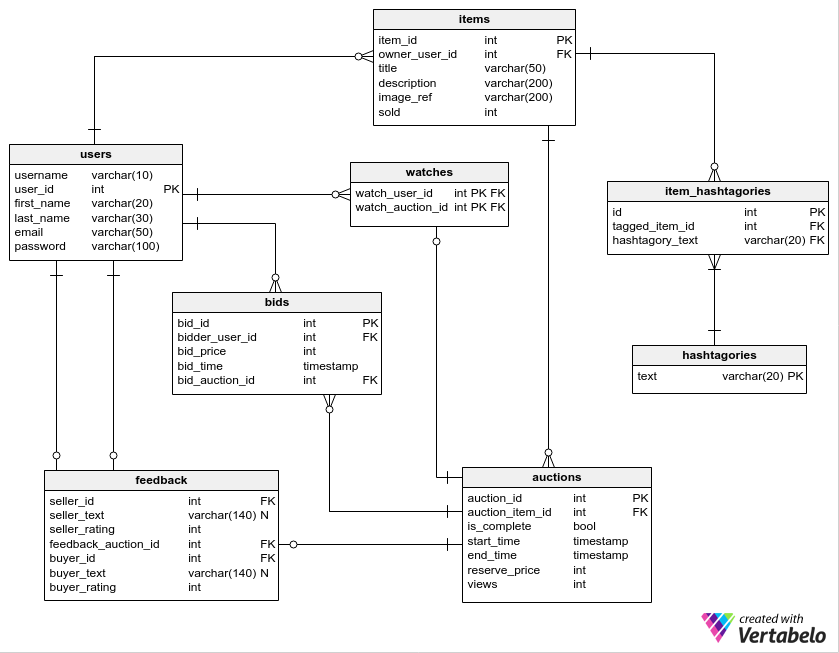
\includegraphics{auction-erd.png}
\caption{alt text}
\end{figure}

\subsection{Database Schema Listing}\label{database-schema-listing}

\subsubsection{Tables}\label{tables}

(Notes in brackets; PK = Primary Key, FK = Foreign Key)

\begin{itemize}
\tightlist
\item
  users

  \begin{itemize}
  \tightlist
  \item
    user\_id (PK)
  \item
    username
  \item
    first\_name
  \item
    last\_name
  \item
    email
  \item
    password (hashed)
  \end{itemize}
\item
  items

  \begin{itemize}
  \tightlist
  \item
    item\_id (PK)
  \item
    owner\_user\_id (FK)
  \item
    title
  \item
    description
  \item
    image\_ref
  \item
    sold
  \end{itemize}
\item
  hashtagories

  \begin{itemize}
  \tightlist
  \item
    id (PK)
  \item
    text (indexed)
  \end{itemize}
\item
  item\_hashtagories

  \begin{itemize}
  \tightlist
  \item
    id (PK)
  \item
    tagged\_item\_id (FK)
  \item
    hashtagory\_text (FK, FULLTEXT indexed)
  \end{itemize}
\item
  auctions

  \begin{itemize}
  \tightlist
  \item
    auction\_id (PK)
  \item
    auction\_item\_id (FK)
  \item
    is\_complete
  \item
    start\_time
  \item
    end\_time
  \item
    reserve\_price
  \item
    views
  \end{itemize}
\item
  bids

  \begin{itemize}
  \tightlist
  \item
    bid\_id (PK)
  \item
    bidder\_user\_id (FK)
  \item
    bid\_price
  \item
    bid\_time
  \item
    bid\_auction\_id (FK)
  \end{itemize}
\item
  watches

  \begin{itemize}
  \tightlist
  \item
    watch\_user\_id (PK, FK)
  \item
    watch\_auction\_id (PK, FK)
  \end{itemize}
\item
  feedback

  \begin{itemize}
  \tightlist
  \item
    feedback\_auction\_id (PK, FK)
  \item
    seller\_id (FK)
  \item
    buyer\_id (FK)
  \item
    buyer\_text
  \item
    seller\_text
  \item
    buyer\_rating
  \item
    seller\_rating
  \end{itemize}
\end{itemize}

\subsubsection{Foreign Key
Relationships}\label{foreign-key-relationships}

The database features a number of foreign key constraints to ensure
referential integrity. The foreign key relationships are summarised in
the following chart, a reduced ERD showing only the properties of each
entity which are involved in constraints:

\begin{figure}[htbp]
\centering
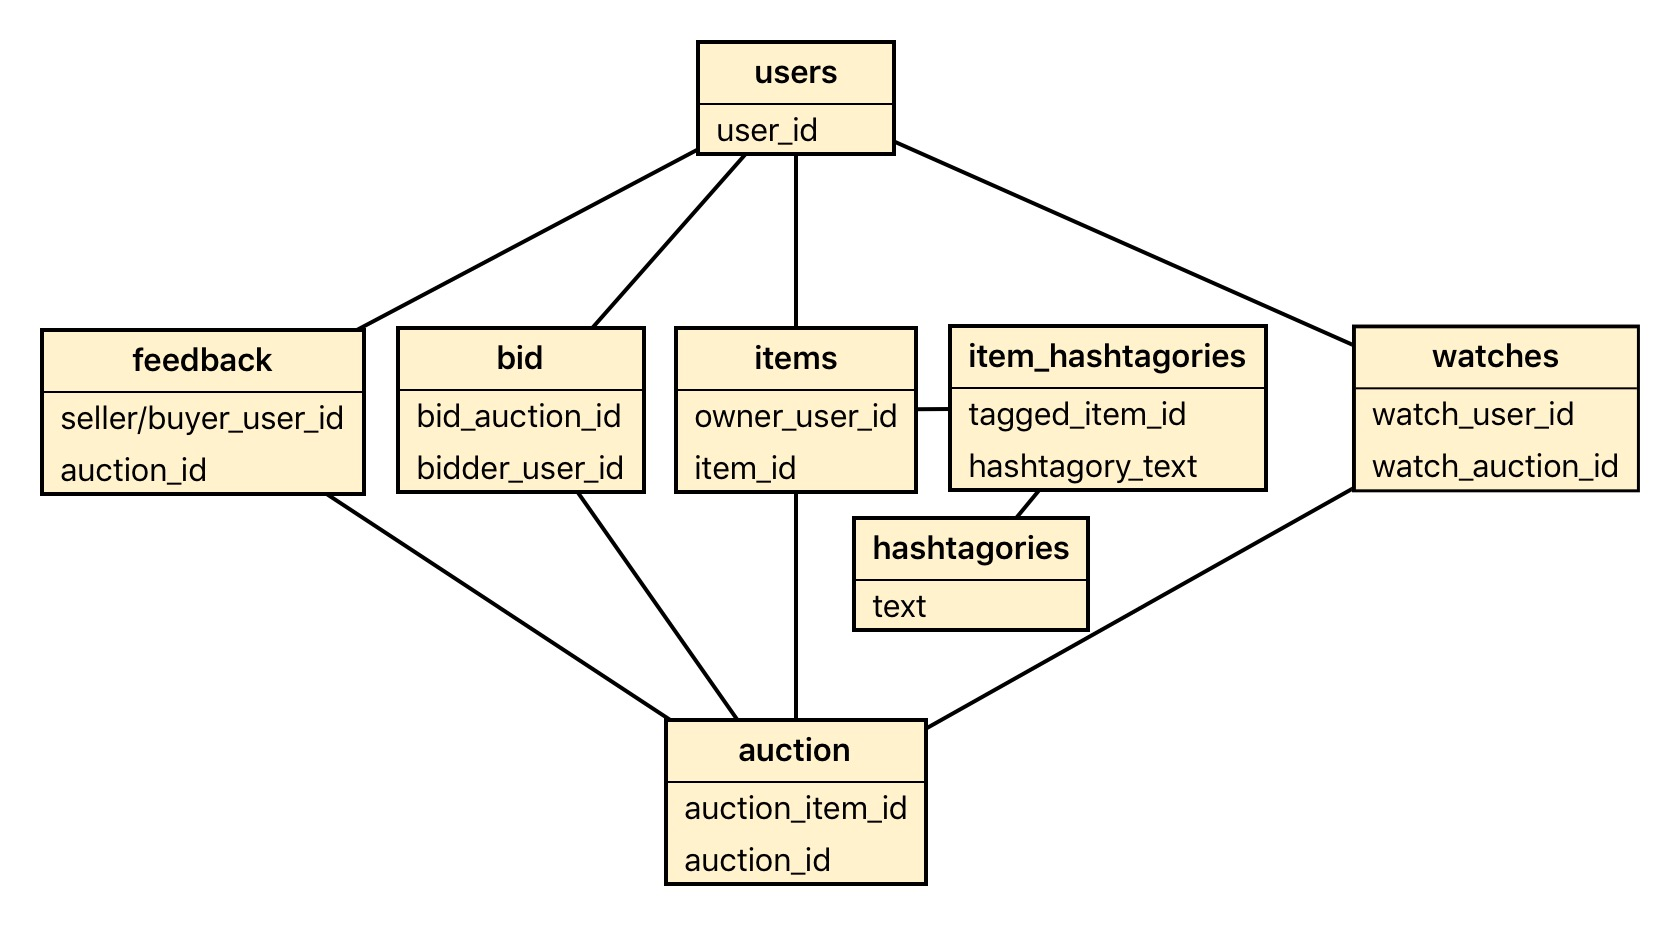
\includegraphics{Fk-diagram.jpeg}
\caption{fk-chart}
\end{figure}

This chart shows the sequence of foreign key dependencies. As can be
seen, the \texttt{users} and the \texttt{hashtagories} tables are the
only table with no foreign key dependencies, and the
\texttt{item\_hashtagories} table is composed entirely of foreign key
fields.

\subsubsection{Additional Schema
Details}\label{additional-schema-details}

In addition to the standard schema definitions, our schema also makes
use of the following techniques:

\begin{itemize}
\tightlist
\item
  MySQL \texttt{STORED\ PROCEDURES}

  \begin{itemize}
  \tightlist
  \item
    Every query used in the application is implemented through one or
    more stored procedures. This provides additional safety from SQL
    injection, as well as allowing the database engine to optimise the
    procedure's query plan. Additionally, many API endpoints utilise the
    same stored procedure, meaning any query changes or adjustments can
    be made in a single location; this provides an efficient layer of
    abstraction.
  \end{itemize}
\item
  A MySQL \texttt{VIEW}, entitled \texttt{auctions\_retrieve\_all}

  \begin{itemize}
  \tightlist
  \item
    This view is used frequently to retrieve composited information
    about all current auctions, or a subset of all current auctions (a
    search)
  \end{itemize}
\item
  MySQL \texttt{FULLTEXT} binary searching, on the
  \texttt{item\_hashtagories} table

  \begin{itemize}
  \tightlist
  \item
    This was employed to allow matching of multiple partial strings to
    multiple partial values (eg. a search for ``table chair'', modified
    to ``table* chair*'' will return any item tagged with ``table'' or
    ``chair'', as well as ``tables'', ``tabletop'', or ``chairs''.
    \texttt{FULLTEXT} searching required an additional index on the
    given column.
  \end{itemize}
\end{itemize}

\subsection{Application Architecture}\label{application-architecture}

This project takes advantage of several modern web architecture
paradigms and industry best practices. While some were functionally
unnecessary at the scale of this project, designing for expansion or
scalability is

\begin{itemize}
\tightlist
\item
  Multi-level system achitecture

  \begin{itemize}
  \tightlist
  \item
    Our system is designed in several layers to provide appropriate
    abstraction and encapsulation, allowing for easier debugging and
    design changes. The application layers are:

    \begin{itemize}
    \tightlist
    \item
      An AngularJS browser-based single-page application
    \item
      A PHP HTTP REST API (that's a lot of acronyms: PHP HyperText
      Preprocessor HyperText Transfer Protocol Representative State
      Transfer Application Programming Interface)
    \item
      A MySQL database with stored procedures
    \end{itemize}
  \end{itemize}
\item
  Utilising cloud services

  \begin{itemize}
  \tightlist
  \item
    For the entirety of development, our app has been hosted on Amazon
    Web Services virtual servers. In order to aid in rapid deployment, a
    script was developed to automatically update the server-hosted
    application when a new commit was pushed on Github.
  \end{itemize}
\item
  Distributed functionality

  \begin{itemize}
  \tightlist
  \item
    In designing the system deployment, inspiration was taken from
    contemporary, scalable deployment practices. In many large web
    applications, the web server and database server are seperate
    physical or virtual machines, often replicated several times over,
    with traffic routed via a load balancer. We used the
    industry-standard Amazon Web Services tools replicate this structure
    in our application: the web application and REST API are hosted on
    an Amazon EC2 (Elastic Cloud Compute) virtual server, and the MySQL
    database is hosted on an Amazon RDS (Relational Database Service)
    virtual server.
  \end{itemize}
\item
  RESTful HTTP API design

  \begin{itemize}
  \tightlist
  \item
    Inspired by other prolific web APIs, we designed the PHP API in a
    REST standard format. This involves a series of nested endpoints,
    organised in a tree structure; each endpoint performs a given
    database operation, manipulating the retrieved data if necessary,
    and returning it to the caller. These endpoints are often
    parameterised (using URL parameters) to retrieve specific data sets.
    In our project, an example URL request might be: GET
    api/auctions/search?query=table
  \end{itemize}
\item
  Task automation using CRON

  \begin{itemize}
  \tightlist
  \item
    There are two tasks that need to be completed once per minute in
    order to maintain the system's core functionality: completing
    expired auctions (including emailing the seller and the winning
    bidder and opening the feedback portal), and notifying ``watchers''
    of auctions about new bids. Both of these tasks can be triggered via
    an API endpoint - the PHP script runs the necessary stored procedure
    (which performs most of the required logic), and then sends any
    required emails. In order to run these tasks regularly, the server
    uses the Unix application \texttt{cron} to, every minute, send an
    HTTP request via \texttt{curl} to each of these endpoints.
  \end{itemize}
\end{itemize}

\subsection{Normalisation Analysis}\label{normalisation-analysis}

A database is in 3rd normal form if it meets 3 criteria: 1. It contains
only atomic values and there are no repeating groups. 2. All non-key
attributes are fully functional dependent on the primary key. 3. There
is no transitive functional dependency.

\subsubsection{1st Normal Form}\label{st-normal-form}

All of our eight tables contain only atomic values meaning that there
are no elements in any of the tables where the data can be further
broken up. i.e.~username is atomic, email is atomic, an
item\_description is atomic. The database is in first normal form. Also,
any groups related to an entity have been separated in a separate table
such as a the hashtagories table.

\subsubsection{2nd Normal Form}\label{nd-normal-form}

This means that in every table in the database a value of a particular
non-key field cannot be uniquely identified via another non-key or group
of non-key fields. Attribute B is dependent on attribute A, but not on a
proper subset of A, then B is fully functional dependent on A. For
example, item\_description can not be uniquely identified by an proper
subset of the item\_id such as title or owner\_user\_id.

\subsubsection{3rd Normal Form}\label{rd-normal-form}

A transitive dependency is when a non-key attribute, C, is dependent on
another attribute, A, via an attribute, B. Our database contains no
transitive dependencies as we put all key attributes that are functional
dependent on another attribute as primary keys in different tables. One
transitive dependency may have occurred if we stored the
hashtagories\_text on the items table, as then the hashtagories\_text
would've been dependent on item\_id via item\_description and therefore
transitively dependent. To avoid this we separated an items hashtagories
tags into a separate table.

\subsubsection{Table of normalisation}\label{table-of-normalisation}

By analysing the attributes in tables of the database we ensured that
none of the attributes break the rules of normalisation. As the table
below indicates, all the tables in the database meet all the
requirements of 3rd normalisation.

\begin{longtable}[c]{@{}llll@{}}
\toprule
Attribute Name & 1st Normal Form & 2nd Normal Form & 3rd Normal
Form\tabularnewline
\midrule
\endhead
\textbf{users} & yes & yes & yes\tabularnewline
\textbf{items} & yes & yes & yes\tabularnewline
\textbf{hashtagories} & yes & yes & yes\tabularnewline
\textbf{item\_hashtagories} & yes & yes & yes\tabularnewline
\textbf{auctions} & yes & yes & yes\tabularnewline
\textbf{bids} & yes & yes & yes\tabularnewline
\textbf{watches} & yes & yes & yes\tabularnewline
\textbf{feedback} & yes & yes & yes\tabularnewline
\bottomrule
\end{longtable}

\subsection{Query Explainations}\label{query-explainations}

Below are all SQL queries used by the system. In writing them as stored
procedures, we have encapsulated their functionality and hopefully
improved readability and modularity/extensibility. Furthermore, because
stored procedures can be parameterised and all parameters are passed as
data, we are insulated against more common SQL injection attacts.
Arguably, it gives better performance as the database does not have to
interpret a SQL string from PHP every time it is called (they are
already stored in executable form), however the speed impact of this is
debated. Please refer to
\href{https://docs.oracle.com/cd/F49540_01/DOC/java.815/a64686/01_intr3.htm}{here}
and
\href{http://sqlblog.com/blogs/paul_nielsen/archive/2009/05/09/why-use-stored-procedures.aspx}{here}
for a more detailed discussion of stored procedures.

This also ensures that the middleware is very light-weight, simply
passing data to and from the front-end via PHP scripts that call stored
procedures.

Additionally, we make use of events for repeated tasks, to prevent the
middleware from having to call the database regularly and hence consume
the connections. We also make use of one view for the sake of
performance (auctions\_retrieve\_all).

\paragraph{auctions\_cancel}\label{auctionsux5fcancel}

Cancels an auction by deleting it from the auction table.

\begin{Shaded}
\begin{Highlighting}[]
\KeywordTok{PROCEDURE} \NormalTok{`auctions_cancel`(}\KeywordTok{IN} \NormalTok{auction_id }\DataTypeTok{INT}\NormalTok{(}\DecValTok{11}\NormalTok{))}
\KeywordTok{BEGIN}
    \KeywordTok{DELETE} \KeywordTok{FROM} \NormalTok{`auctions` }\KeywordTok{WHERE} \NormalTok{auctions.auction_id = auction_id;}
\KeywordTok{END}
\end{Highlighting}
\end{Shaded}

\paragraph{auctions\_create}\label{auctionsux5fcreate}

Starts an auction, using timestamps generated in the middle-layer (could
have also used NOW() function). Reserve price needs to be cast from
string input.

\begin{Shaded}
\begin{Highlighting}[]
\KeywordTok{PROCEDURE} \NormalTok{`auctions_create`(}\KeywordTok{IN} \NormalTok{auction_item_id }\DataTypeTok{INT}\NormalTok{(}\DecValTok{11}\NormalTok{), }\KeywordTok{IN} \NormalTok{start_time }\DataTypeTok{timestamp}\NormalTok{, }\KeywordTok{IN} \NormalTok{end_time }\DataTypeTok{timestamp}\NormalTok{, }\KeywordTok{IN} \NormalTok{reserve_price }\DataTypeTok{varchar}\NormalTok{(}\DecValTok{12}\NormalTok{))}
\KeywordTok{BEGIN}
    \KeywordTok{INSERT} \KeywordTok{INTO} \NormalTok{`auctions` (auctions.auction_item_id, auctions.start_time, auctions.end_time, auctions.reserve_price)  }
    \KeywordTok{VALUES}\NormalTok{(auction_item_id, start_time, end_time, }\FunctionTok{CAST}\NormalTok{(reserve_price }\KeywordTok{AS} \DataTypeTok{DECIMAL}\NormalTok{(}\DecValTok{10}\NormalTok{,}\DecValTok{2}\NormalTok{)));}
    \KeywordTok{SELECT} \NormalTok{last_insert_id();}
\KeywordTok{END}
\end{Highlighting}
\end{Shaded}

\paragraph{auctions\_retrieve\_all}\label{auctionsux5fretrieveux5fall}

This stored procedure shows a set of auction objects with user name,
item details and auction details, as well as highest bid. This is
actually achieved by selecting from a view (code below). Note: Highest
bids needed to be selected into a subtable and then joined to cope with
some auctions not having bids placed.

\begin{Shaded}
\begin{Highlighting}[]
\KeywordTok{PROCEDURE} \NormalTok{`auctions_retrieve_all`()}
\KeywordTok{BEGIN}
    \KeywordTok{SELECT} \NormalTok{* }\KeywordTok{FROM} \NormalTok{auctions_retrieve_all;}
\KeywordTok{END}

\NormalTok{#View creation}
\KeywordTok{CREATE} \KeywordTok{TABLE} \NormalTok{`auctions_retrieve_all` (}
   \NormalTok{`auction_id` }\DataTypeTok{INT}\NormalTok{(}\DecValTok{11}\NormalTok{) }\KeywordTok{NOT} \KeywordTok{NULL} \KeywordTok{DEFAULT} \StringTok{'0'}\NormalTok{,}
   \NormalTok{`auction_item_id` }\DataTypeTok{INT}\NormalTok{(}\DecValTok{11}\NormalTok{) }\KeywordTok{NOT} \KeywordTok{NULL}\NormalTok{,}
   \NormalTok{`is_complete` TINYINT(}\DecValTok{1}\NormalTok{) }\KeywordTok{NOT} \KeywordTok{NULL} \KeywordTok{DEFAULT} \StringTok{'0'}\NormalTok{,}
   \NormalTok{`start_time` }\DataTypeTok{TIMESTAMP} \KeywordTok{NOT} \KeywordTok{NULL}\NormalTok{,}
   \NormalTok{`end_time` }\DataTypeTok{TIMESTAMP} \KeywordTok{NOT} \KeywordTok{NULL}\NormalTok{,}
   \NormalTok{`reserve_price` }\DataTypeTok{DECIMAL}\NormalTok{(}\DecValTok{10}\NormalTok{) }\KeywordTok{NOT} \KeywordTok{NULL}\NormalTok{,}
   \NormalTok{`views` }\DataTypeTok{INT}\NormalTok{(}\DecValTok{11}\NormalTok{) UNSIGNED ZEROFILL }\KeywordTok{NOT} \KeywordTok{NULL} \KeywordTok{DEFAULT} \StringTok{'00000000000'}\NormalTok{,}
   \NormalTok{`current_bid` }\DataTypeTok{DECIMAL}\NormalTok{(}\DecValTok{10}\NormalTok{) }\KeywordTok{NULL} \KeywordTok{DEFAULT} \KeywordTok{NULL}\NormalTok{,}
   \NormalTok{`item_id` }\DataTypeTok{INT}\NormalTok{(}\DecValTok{11}\NormalTok{) }\KeywordTok{NULL} \KeywordTok{DEFAULT} \StringTok{'0'}\NormalTok{,}
   \NormalTok{`owner_user_id` }\DataTypeTok{INT}\NormalTok{(}\DecValTok{11}\NormalTok{) }\KeywordTok{NULL} \KeywordTok{DEFAULT} \KeywordTok{NULL}\NormalTok{,}
   \NormalTok{`title` }\DataTypeTok{VARCHAR}\NormalTok{(}\DecValTok{50}\NormalTok{) }\KeywordTok{NULL} \KeywordTok{DEFAULT} \StringTok{''}\NormalTok{,}
   \NormalTok{`description` }\DataTypeTok{VARCHAR}\NormalTok{(}\DecValTok{200}\NormalTok{) }\KeywordTok{NULL} \KeywordTok{DEFAULT} \StringTok{''}\NormalTok{,}
   \NormalTok{`image_ref` }\DataTypeTok{VARCHAR}\NormalTok{(}\DecValTok{255}\NormalTok{) }\KeywordTok{NULL} \KeywordTok{DEFAULT} \KeywordTok{NULL}\NormalTok{,}
   \NormalTok{`sold` }\DataTypeTok{INT}\NormalTok{(}\DecValTok{1}\NormalTok{) }\KeywordTok{NULL} \KeywordTok{DEFAULT} \StringTok{'0'}\NormalTok{,}
   \NormalTok{`username` }\DataTypeTok{VARCHAR}\NormalTok{(}\DecValTok{10}\NormalTok{) }\KeywordTok{NULL} \KeywordTok{DEFAULT} \KeywordTok{NULL}
\NormalTok{) ENGINE=MyISAM;}
\end{Highlighting}
\end{Shaded}

\paragraph{auctions\_search}\label{auctionsux5fsearch}

Allows for a partial search of auctions, returning auction items with
item and user details, sorted in a variety of modes. The stored
procedure is also structured in such a way that it returns the full
result set of all open auctions sorted in the way specified by the sort
parameter. This allows us to use a single end-point to display both feed
and search data sorted in the requisite order.

\begin{Shaded}
\begin{Highlighting}[]
\KeywordTok{PROCEDURE} \NormalTok{`auctions_search`(}\KeywordTok{IN} \NormalTok{str }\DataTypeTok{varchar}\NormalTok{(}\DecValTok{100}\NormalTok{), }\KeywordTok{IN} \KeywordTok{sort} \DataTypeTok{varchar}\NormalTok{(}\DecValTok{10}\NormalTok{))}
\KeywordTok{BEGIN}
    \KeywordTok{SELECT} \NormalTok{*}
    \KeywordTok{FROM} \NormalTok{item_hashtagories }\KeywordTok{AS} \NormalTok{ih, auctions_retrieve_all }\KeywordTok{AS} \NormalTok{a}
    
    \KeywordTok{WHERE} \NormalTok{(str = }\StringTok{''} \KeywordTok{OR} \NormalTok{MATCH(ih.hashtagory_text) AGAINST(str }\KeywordTok{IN} \DataTypeTok{BOOLEAN} \KeywordTok{MODE}\NormalTok{))}
        \KeywordTok{AND} \NormalTok{ih.tagged_item_id = a.item_id}
    \KeywordTok{GROUP} \KeywordTok{BY} \NormalTok{a.auction_id}
    \KeywordTok{ORDER} \KeywordTok{BY} \KeywordTok{CASE} \KeywordTok{sort}
                \KeywordTok{when} \StringTok{'start_time'} \KeywordTok{then} \NormalTok{a.start_time}
                \KeywordTok{when} \StringTok{'end_time'} \KeywordTok{then} \NormalTok{a.end_time}
                \KeywordTok{when} \StringTok{'views'} \KeywordTok{then} \NormalTok{a.views}
                \KeywordTok{when} \StringTok{'title'} \KeywordTok{then} \NormalTok{a.title}
            \KeywordTok{END}
        \NormalTok{;}

\KeywordTok{END}
\end{Highlighting}
\end{Shaded}

\paragraph{auctions\_search\_desc}\label{auctionsux5fsearchux5fdesc}

Mirror of previous search procedure with descending sorting. This
minimised the parameters that needed to be passed through the middleware
(the PHP endpoints select which procedure to call based on a sorting
parameter passed from the front-end).

\begin{Shaded}
\begin{Highlighting}[]
\KeywordTok{PROCEDURE} \NormalTok{`auctions_search_desc`(}\KeywordTok{IN} \NormalTok{str }\DataTypeTok{varchar}\NormalTok{(}\DecValTok{100}\NormalTok{), }\KeywordTok{IN} \KeywordTok{sort} \DataTypeTok{varchar}\NormalTok{(}\DecValTok{10}\NormalTok{))}
\KeywordTok{BEGIN}
    \KeywordTok{SELECT} \KeywordTok{DISTINCT} \NormalTok{*}
    \KeywordTok{FROM} \NormalTok{item_hashtagories }\KeywordTok{AS} \NormalTok{ih, auctions_retrieve_all }\KeywordTok{AS} \NormalTok{a}
    
    \KeywordTok{WHERE} \NormalTok{(str = }\StringTok{''} \KeywordTok{OR} \NormalTok{MATCH(ih.hashtagory_text) AGAINST(str }\KeywordTok{IN} \DataTypeTok{BOOLEAN} \KeywordTok{MODE}\NormalTok{))}
        \KeywordTok{AND} \NormalTok{ih.tagged_item_id = a.item_id}
    \KeywordTok{GROUP} \KeywordTok{BY} \NormalTok{a.auction_id}
    \KeywordTok{ORDER} \KeywordTok{BY} \KeywordTok{CASE} \KeywordTok{sort}
                \KeywordTok{when} \StringTok{'start_time'} \KeywordTok{then} \NormalTok{a.start_time}
                \KeywordTok{when} \StringTok{'end_time'} \KeywordTok{then} \NormalTok{a.end_time}
                \KeywordTok{when} \StringTok{'views'} \KeywordTok{then} \NormalTok{a.views}
                \KeywordTok{when} \StringTok{'title'} \KeywordTok{then} \NormalTok{a.title}
            \KeywordTok{END}
            \KeywordTok{DESC}
        \NormalTok{;}
\KeywordTok{END}
\end{Highlighting}
\end{Shaded}

\paragraph{auctions\_self}\label{auctionsux5fself}

Returns the information about a particular auction (bids are pulled in
seperately for display purposes). Also updates the view field of the
auction record, as this procedure is always called every time an auction
is viewed.

\begin{Shaded}
\begin{Highlighting}[]
\NormalTok{PROCEDURE`auctions_self`(}\KeywordTok{IN} \NormalTok{auction_id }\DataTypeTok{INT}\NormalTok{(}\DecValTok{11}\NormalTok{))}
\KeywordTok{BEGIN}
\KeywordTok{UPDATE} \NormalTok{auctions }\KeywordTok{SET} \NormalTok{auctions.views = auctions.views}\DecValTok{+1} \KeywordTok{WHERE} \NormalTok{auctions.auction_id = auction_id;}
\KeywordTok{SELECT} \NormalTok{items.*, users.username, auctions.* }\KeywordTok{FROM} \NormalTok{`auctions`}
    \KeywordTok{LEFT} \KeywordTok{JOIN} \NormalTok{`items` }\KeywordTok{ON} \NormalTok{auctions.auction_item_id = items.item_id}
    \KeywordTok{LEFT} \KeywordTok{JOIN} \NormalTok{`users` }\KeywordTok{ON} \NormalTok{items.owner_user_id = users.user_id}
    \KeywordTok{WHERE} \NormalTok{auctions.auction_id = auction_id;}
\KeywordTok{END}
\end{Highlighting}
\end{Shaded}

\paragraph{auctions\_user\_auctions}\label{auctionsux5fuserux5fauctions}

Returns all auctions created by a particular user.

\begin{Shaded}
\begin{Highlighting}[]
\KeywordTok{PROCEDURE} \NormalTok{`auctions_user_auctions`(}\KeywordTok{IN} \NormalTok{user_id }\DataTypeTok{INT}\NormalTok{(}\DecValTok{11}\NormalTok{))}
\KeywordTok{BEGIN}
    \KeywordTok{SELECT} \NormalTok{* }\KeywordTok{FROM} \NormalTok{`auctions` }\KeywordTok{AS} \NormalTok{a, `items` }\KeywordTok{AS} \NormalTok{i}
    \KeywordTok{WHERE} \NormalTok{a.is_complete = }\DecValTok{0}
    \KeywordTok{AND} \NormalTok{a.auction_item_id = i.item_id}
    \KeywordTok{AND} \NormalTok{i.owner_user_id = user_id}
    \KeywordTok{ORDER} \KeywordTok{BY} \NormalTok{`end_time` }\KeywordTok{ASC}\NormalTok{;}
\KeywordTok{END}
\end{Highlighting}
\end{Shaded}

\paragraph{auctions\_user\_feed}\label{auctionsux5fuserux5ffeed}

Returns a feed of auctions relevant to the bids that they have made.

\begin{Shaded}
\begin{Highlighting}[]
\KeywordTok{PROCEDURE} \NormalTok{`auctions_user_feed`(}\KeywordTok{IN} \NormalTok{user_id }\DataTypeTok{INT}\NormalTok{(}\DecValTok{11}\NormalTok{))}
\KeywordTok{BEGIN}
    \KeywordTok{SELECT} \NormalTok{* }\KeywordTok{FROM} \NormalTok{auctions }\KeywordTok{as} \NormalTok{a}
    \KeywordTok{LEFT} \KeywordTok{JOIN} \NormalTok{items }\KeywordTok{as} \NormalTok{i }\KeywordTok{ON} \NormalTok{a.auction_item_id = i.item_id}
    \KeywordTok{LEFT} \KeywordTok{JOIN} \NormalTok{bids }\KeywordTok{as} \NormalTok{b }\KeywordTok{ON} \NormalTok{a.auction_id = b.bid_auction_id}
    \KeywordTok{WHERE} \NormalTok{b.bidder_user_id = user_id }\KeywordTok{AND} \NormalTok{a.is_complete = }\DecValTok{0}
    \KeywordTok{ORDER} \KeywordTok{BY} \NormalTok{a.end_time }\KeywordTok{ASC}\NormalTok{;}
\KeywordTok{END}
\end{Highlighting}
\end{Shaded}

\paragraph{bids\_auction\_bids}\label{bidsux5fauctionux5fbids}

Returns the set of bids on any given auction.

\begin{Shaded}
\begin{Highlighting}[]
\KeywordTok{PROCEDURE} \NormalTok{`bids_auction_bids`(}\KeywordTok{IN} \NormalTok{bid_auction_id }\DataTypeTok{INT}\NormalTok{(}\DecValTok{11}\NormalTok{))}
\KeywordTok{BEGIN}
    \KeywordTok{SELECT} \NormalTok{* }\KeywordTok{FROM} \NormalTok{bids }\KeywordTok{WHERE} \NormalTok{bids.bid_auction_id = bid_auction_id}
    \KeywordTok{ORDER} \KeywordTok{BY} \NormalTok{bids.bid_price }\KeywordTok{DESC}\NormalTok{;}
\KeywordTok{END}
\end{Highlighting}
\end{Shaded}

\paragraph{bids\_create}\label{bidsux5fcreate}

Procedure called when bid is placed on item. Bid value validation (that
new bid is the higest) can be performed on the front-end and is also
duplicated here. Here, the stored procedure first checks the highest bid
against the attempted bid, and only inserts the bid if it is higher. It
will also add the auction the the user's watchlist by calling the stored
procedure.

\begin{Shaded}
\begin{Highlighting}[]
\KeywordTok{PROCEDURE} \NormalTok{`bids_create`( }\KeywordTok{IN} \NormalTok{bidder_user_id }\DataTypeTok{INT}\NormalTok{(}\DecValTok{11}\NormalTok{), }\KeywordTok{IN} \NormalTok{bid_price }\DataTypeTok{VARCHAR}\NormalTok{(}\DecValTok{12}\NormalTok{), }\KeywordTok{IN} \NormalTok{bid_auction_id }\DataTypeTok{INT}\NormalTok{)}
\KeywordTok{BEGIN}
    \KeywordTok{DECLARE} \NormalTok{highest_bid }\DataTypeTok{DECIMAL}\NormalTok{(}\DecValTok{10}\NormalTok{,}\DecValTok{2}\NormalTok{) }\KeywordTok{DEFAULT} \DecValTok{0}\NormalTok{;}

    \KeywordTok{SELECT} \NormalTok{bid_price }\KeywordTok{FROM} \NormalTok{`bids` }\KeywordTok{WHERE} \NormalTok{bids.bid_auction_id = bid_auction_id }\KeywordTok{ORDER} \KeywordTok{BY} \NormalTok{bid_price }\KeywordTok{DESC} \KeywordTok{LIMIT} \DecValTok{1} \KeywordTok{INTO} \NormalTok{highest_bid;}

    \KeywordTok{SELECT} \NormalTok{bid_price_in, highest_bid;}
    \KeywordTok{IF} \NormalTok{bid_price_in > highest_bid }\KeywordTok{THEN}

    \KeywordTok{INSERT} \KeywordTok{INTO} \NormalTok{`bids` (bids.bidder_user_id, bids.bid_price, bids.bid_time, bids.bid_auction_id)}
        \KeywordTok{VALUES}\NormalTok{(bidder_user_id, }\FunctionTok{CAST}\NormalTok{(bid_price_in }\KeywordTok{AS} \DataTypeTok{DECIMAL}\NormalTok{(}\DecValTok{10}\NormalTok{,}\DecValTok{2}\NormalTok{)), NOW(), bid_auction_id);}
    \KeywordTok{SELECT} \NormalTok{last_insert_id();}
\KeywordTok{ELSE}
     \NormalTok{SIGNAL SQLSTATE }\StringTok{'45000'} \KeywordTok{SET} \NormalTok{MESSAGE_TEXT = }\StringTok{'Bid price too low!'}\NormalTok{;}
\KeywordTok{IF}\NormalTok{;}
    \KeywordTok{CALL} \NormalTok{watches_create(bidder_user_id, bid_auction_id);}
\KeywordTok{END}
\end{Highlighting}
\end{Shaded}

\paragraph{bids\_self}\label{bidsux5fself}

Returns the auction that a bid is related to.

\begin{Shaded}
\begin{Highlighting}[]
\KeywordTok{PROCEDURE} \NormalTok{`bids_self`(}\KeywordTok{IN} \NormalTok{bid_id }\DataTypeTok{INT}\NormalTok{(}\DecValTok{11}\NormalTok{))}
\KeywordTok{BEGIN}
    \KeywordTok{SELECT} \NormalTok{* }\KeywordTok{FROM} \NormalTok{auctions }\KeywordTok{AS} \NormalTok{a}
    \KeywordTok{LEFT} \KeywordTok{JOIN} \NormalTok{items }\KeywordTok{AS} \NormalTok{i }\KeywordTok{ON} \NormalTok{a.auction_item_id = i.item_id}
    \KeywordTok{LEFT} \KeywordTok{JOIN} \NormalTok{bids }\KeywordTok{as} \NormalTok{b }\KeywordTok{ON} \NormalTok{a.auction_id = b.bid_auction_id}
    \KeywordTok{WHERE} \NormalTok{b.bid_id = bid_id;}
\KeywordTok{END}
\end{Highlighting}
\end{Shaded}

\paragraph{bids\_user\_bids}\label{bidsux5fuserux5fbids}

Returns auction data objects on which a given user has bid (auction
details, item deails and bid details).

\begin{Shaded}
\begin{Highlighting}[]
\KeywordTok{PROCEDURE} \NormalTok{`bids_user_bids`(}\KeywordTok{IN} \NormalTok{user_id }\DataTypeTok{INT}\NormalTok{(}\DecValTok{11}\NormalTok{))}
\KeywordTok{BEGIN}
    \KeywordTok{SELECT} \NormalTok{a.*, b.*, i.*, u.username }\KeywordTok{FROM} \NormalTok{users }\KeywordTok{AS} \NormalTok{u, auctions }\KeywordTok{AS} \NormalTok{a}
    \KeywordTok{LEFT} \KeywordTok{JOIN} \NormalTok{items }\KeywordTok{AS} \NormalTok{i }\KeywordTok{ON} \NormalTok{a.auction_item_id = i.item_id}
    \KeywordTok{LEFT} \KeywordTok{JOIN} \NormalTok{bids }\KeywordTok{AS} \NormalTok{b }\KeywordTok{ON} \NormalTok{a.auction_id = b.bid_auction_id}
    \KeywordTok{WHERE} \NormalTok{user_id = b.bidder_user_id }\KeywordTok{AND} \NormalTok{i.owner_user_id = u.user_id }
    \KeywordTok{ORDER} \KeywordTok{BY} \NormalTok{b.bid_time }\KeywordTok{DESC}\NormalTok{;}
\KeywordTok{END}
\end{Highlighting}
\end{Shaded}

\paragraph{event\_end\_expired\_auctions}\label{eventux5fendux5fexpiredux5fauctions}

Ends all expired auctions and returns the data on the auctions such as
the buyer, seller, name, winning bid etc. By running the event on a
timer, the database does not need to have its connection tied up by an
automated call from the API.

\begin{Shaded}
\begin{Highlighting}[]
\KeywordTok{PROCEDURE} \NormalTok{`event_end_expired_auctions`()}
\KeywordTok{BEGIN}

    \KeywordTok{DECLARE} \NormalTok{reserve_price_tmp }\DataTypeTok{INT} \KeywordTok{DEFAULT} \DecValTok{0}\NormalTok{;}
    \KeywordTok{DECLARE} \NormalTok{highest_bid_tmp }\DataTypeTok{decimal}\NormalTok{(}\DecValTok{10}\NormalTok{,}\DecValTok{2}\NormalTok{) }\KeywordTok{DEFAULT} \DecValTok{0}\NormalTok{;}
    \KeywordTok{DECLARE} \NormalTok{auction_id_tmp }\DataTypeTok{INT} \KeywordTok{DEFAULT} \DecValTok{0}\NormalTok{;}

    \KeywordTok{DECLARE} \NormalTok{item_title_tmp }\DataTypeTok{varchar}\NormalTok{(}\DecValTok{200}\NormalTok{) }\KeywordTok{DEFAULT} \DecValTok{0}\NormalTok{;}
    \KeywordTok{DECLARE} \NormalTok{item_id_tmp }\DataTypeTok{INT} \KeywordTok{DEFAULT} \DecValTok{0}\NormalTok{;}

    \KeywordTok{DECLARE} \NormalTok{seller_url_tmp }\DataTypeTok{varchar}\NormalTok{(}\DecValTok{200}\NormalTok{) }\KeywordTok{DEFAULT} \DecValTok{0}\NormalTok{;}
    \KeywordTok{DECLARE} \NormalTok{buyer_url_tmp }\DataTypeTok{varchar}\NormalTok{(}\DecValTok{200}\NormalTok{) }\KeywordTok{DEFAULT} \DecValTok{0}\NormalTok{;}
    \KeywordTok{DECLARE} \NormalTok{seller_username_tmp }\DataTypeTok{varchar}\NormalTok{(}\DecValTok{200}\NormalTok{) }\KeywordTok{DEFAULT} \DecValTok{0}\NormalTok{;}
    \KeywordTok{DECLARE} \NormalTok{buyer_username_tmp }\DataTypeTok{varchar}\NormalTok{(}\DecValTok{200}\NormalTok{) }\KeywordTok{DEFAULT} \DecValTok{0}\NormalTok{;}
    \KeywordTok{DECLARE} \NormalTok{seller_email_tmp }\DataTypeTok{varchar}\NormalTok{(}\DecValTok{200}\NormalTok{) }\KeywordTok{DEFAULT} \DecValTok{0}\NormalTok{;}
    \KeywordTok{DECLARE} \NormalTok{buyer_email_tmp }\DataTypeTok{varchar}\NormalTok{(}\DecValTok{200}\NormalTok{) }\KeywordTok{DEFAULT} \DecValTok{0}\NormalTok{;}
    \KeywordTok{DECLARE} \NormalTok{seller_id_tmp }\DataTypeTok{INT} \KeywordTok{DEFAULT} \DecValTok{0}\NormalTok{;}
    \KeywordTok{DECLARE} \NormalTok{buyer_id_tmp }\DataTypeTok{INT} \KeywordTok{DEFAULT} \DecValTok{0}\NormalTok{;}

    \KeywordTok{DECLARE} \NormalTok{successful_tmp }\DataTypeTok{INT} \KeywordTok{DEFAULT} \DecValTok{0}\NormalTok{;}

    \KeywordTok{DECLARE} \NormalTok{n }\DataTypeTok{INT} \KeywordTok{DEFAULT} \DecValTok{0}\NormalTok{;}
    \KeywordTok{DECLARE} \NormalTok{i }\DataTypeTok{INT} \KeywordTok{DEFAULT} \DecValTok{0}\NormalTok{;}

        \NormalTok{# Drops }\KeywordTok{the} \KeywordTok{temporary} \KeywordTok{table} \KeywordTok{if} \NormalTok{it exists. }\KeywordTok{Then} \NormalTok{creates it.}
        \KeywordTok{DROP} \KeywordTok{TABLE} \KeywordTok{IF} \KeywordTok{EXISTS} \NormalTok{`tmp_end_expired_auctions`;}
        \KeywordTok{CREATE} \KeywordTok{TABLE} \NormalTok{`tmp_end_expired_auctions` (}
          \NormalTok{`auction_id` }\DataTypeTok{int}\NormalTok{(}\DecValTok{11}\NormalTok{) }\KeywordTok{NOT} \KeywordTok{NULL}\NormalTok{,}
          \NormalTok{`seller_username` }\DataTypeTok{varchar}\NormalTok{(}\DecValTok{200}\NormalTok{) }\KeywordTok{DEFAULT} \KeywordTok{NULL}\NormalTok{,}
          \NormalTok{`seller_email` }\DataTypeTok{varchar}\NormalTok{(}\DecValTok{200}\NormalTok{) }\KeywordTok{DEFAULT} \KeywordTok{NULL}\NormalTok{,}
          \NormalTok{`seller_feedback_url` }\DataTypeTok{varchar}\NormalTok{(}\DecValTok{50}\NormalTok{) }\KeywordTok{DEFAULT} \KeywordTok{NULL}\NormalTok{,}
          \NormalTok{`buyer_username` }\DataTypeTok{varchar}\NormalTok{(}\DecValTok{200}\NormalTok{) }\KeywordTok{DEFAULT} \KeywordTok{NULL}\NormalTok{,}
          \NormalTok{`buyer_email` }\DataTypeTok{varchar}\NormalTok{(}\DecValTok{200}\NormalTok{) }\KeywordTok{DEFAULT} \KeywordTok{NULL}\NormalTok{,}
          \NormalTok{`buyer_feedback_url` }\DataTypeTok{varchar}\NormalTok{(}\DecValTok{50}\NormalTok{) }\KeywordTok{DEFAULT} \KeywordTok{NULL}\NormalTok{,}
          \NormalTok{`item_title` }\DataTypeTok{varchar}\NormalTok{(}\DecValTok{200}\NormalTok{) }\KeywordTok{DEFAULT} \KeywordTok{NULL}\NormalTok{,}
          \NormalTok{`final_bid_price` }\DataTypeTok{varchar}\NormalTok{(}\DecValTok{200}\NormalTok{) }\KeywordTok{DEFAULT} \KeywordTok{NULL}\NormalTok{,}
          \NormalTok{`successful` }\DataTypeTok{varchar}\NormalTok{(}\DecValTok{200}\NormalTok{) }\KeywordTok{DEFAULT} \KeywordTok{NULL}\NormalTok{,}
          \KeywordTok{PRIMARY} \KeywordTok{KEY} \NormalTok{(`auction_id`)}
        \NormalTok{) ENGINE=InnoDB }\KeywordTok{DEFAULT} \NormalTok{CHARSET=latin1;}

        \KeywordTok{SELECT} \FunctionTok{count}\NormalTok{(*) }\KeywordTok{FROM} \NormalTok{`auctions` }\KeywordTok{WHERE} \NormalTok{end_time < now() }\KeywordTok{AND} \NormalTok{is_complete=}\DecValTok{0} \KeywordTok{INTO} \NormalTok{n;    }

        \NormalTok{# This loops }\KeywordTok{through} \KeywordTok{the} \NormalTok{unclosed auctions }\KeywordTok{in} \KeywordTok{the} \NormalTok{auctions }\KeywordTok{table} \KeywordTok{select} \KeywordTok{values}
        \NormalTok{# }\KeywordTok{from} \NormalTok{other tables. It evaluates whether an auction failed }\KeywordTok{or} \NormalTok{was }\KeywordTok{successful}
        \NormalTok{# every }\KeywordTok{loop} \NormalTok{inserts a }\KeywordTok{row} \KeywordTok{to} \KeywordTok{the} \NormalTok{tmp table.}
        \KeywordTok{SET} \NormalTok{i=}\DecValTok{0}\NormalTok{;}
        \KeywordTok{WHILE} \NormalTok{i<n DO }

            \NormalTok{# Auction }\KeywordTok{table} \NormalTok{selects. Gets }\KeywordTok{the} \NormalTok{auction_id, reserver_price }\KeywordTok{and} \NormalTok{item_id.}
            \KeywordTok{SELECT} \NormalTok{auction_id, reserve_price, auction_item_id  }\KeywordTok{FROM} \NormalTok{`auctions` }
            \KeywordTok{WHERE} \NormalTok{end_time < now() }\KeywordTok{AND} \NormalTok{is_complete=}\DecValTok{0} \KeywordTok{ORDER} \KeywordTok{BY} \NormalTok{auction_id }\KeywordTok{LIMIT} \NormalTok{i, }\DecValTok{1} 
                \KeywordTok{INTO} \NormalTok{auction_id_tmp, reserve_price_tmp, item_id_tmp;}

            \NormalTok{# Bids }\KeywordTok{table} \NormalTok{selects. Gets }\KeywordTok{the} \NormalTok{highest_bid }\KeywordTok{on} \NormalTok{an item, }\KeywordTok{and} \KeywordTok{the} \NormalTok{user_id}
            \NormalTok{# }\KeywordTok{of} \NormalTok{that bid.}
            \KeywordTok{SELECT} \NormalTok{bid_price, bidder_user_id }\KeywordTok{FROM} \NormalTok{`bids`}
            \KeywordTok{WHERE} \NormalTok{bid_auction_id = auction_id_tmp }\KeywordTok{ORDER} \KeywordTok{BY} \NormalTok{bid_price }\KeywordTok{DESC} \KeywordTok{LIMIT} \DecValTok{1}
                \KeywordTok{INTO} \NormalTok{highest_bid_tmp, buyer_id_tmp;}

            \NormalTok{# Items }\KeywordTok{table} \NormalTok{selects. Gets }\KeywordTok{the} \NormalTok{user_id }\KeywordTok{of} \KeywordTok{the} \NormalTok{seller }\KeywordTok{and} \KeywordTok{the} \NormalTok{items title.}
            \KeywordTok{SELECT} \NormalTok{owner_user_id, title }\KeywordTok{FROM} \NormalTok{`items` }
            \KeywordTok{WHERE} \NormalTok{item_id = item_id_tmp }\KeywordTok{INTO} \NormalTok{seller_id_tmp, item_title_tmp;}

            \NormalTok{# Users }\KeywordTok{table} \NormalTok{selects seller. Gets seller username }\KeywordTok{and} \NormalTok{email.}
            \KeywordTok{SELECT} \NormalTok{username, email }\KeywordTok{FROM} \NormalTok{`users`}
            \KeywordTok{WHERE} \NormalTok{user_id = seller_id_tmp }\KeywordTok{INTO} \NormalTok{seller_username_tmp, seller_email_tmp;}


            \NormalTok{# }\KeywordTok{If} \NormalTok{it was }\KeywordTok{successful} \KeywordTok{and} \NormalTok{there }\KeywordTok{is} \NormalTok{a buyer user_id}
            \KeywordTok{IF} \NormalTok{buyer_id_tmp > }\DecValTok{0} \KeywordTok{THEN}
                \NormalTok{# Users }\KeywordTok{table} \NormalTok{selects buyer. Gets buyer username }\KeywordTok{and} \NormalTok{email. }
                \KeywordTok{SELECT} \NormalTok{username, email }\KeywordTok{FROM} \NormalTok{`users`}
                \KeywordTok{WHERE} \NormalTok{user_id = buyer_id_tmp }\KeywordTok{INTO} \NormalTok{buyer_username_tmp, buyer_email_tmp;}

            \KeywordTok{END} \KeywordTok{IF}\NormalTok{;}

            \NormalTok{# }\KeywordTok{If} \KeywordTok{successful} \NormalTok{auction: }\KeywordTok{create} \NormalTok{feedback, }\KeywordTok{set} \KeywordTok{successful} \KeywordTok{to} \DecValTok{1}
            \KeywordTok{IF} \NormalTok{highest_bid_tmp >= reserve_price_tmp }\KeywordTok{AND} \NormalTok{highest_bid_tmp > }\DecValTok{0} \KeywordTok{THEN}

                \NormalTok{# }\KeywordTok{Create} \NormalTok{feedback}
                \KeywordTok{INSERT} \NormalTok{IGNORE }\KeywordTok{INTO} \NormalTok{`feedback`}
                    \NormalTok{(`seller_id`,}
                    \NormalTok{`feedback_auction_id`,}
                    \NormalTok{`buyer_id`)}
                    \KeywordTok{VALUES}
                    \NormalTok{(seller_id_tmp,}
                    \NormalTok{auction_id_tmp,}
                    \NormalTok{buyer_id_tmp);}

                \NormalTok{# Sold field }\KeywordTok{in} \NormalTok{items }\KeywordTok{is} \KeywordTok{set} \KeywordTok{to} \KeywordTok{the} \NormalTok{buyer id.}
                \KeywordTok{UPDATE} \NormalTok{`items` }\KeywordTok{SET} \NormalTok{sold = buyer_id_tmp }\KeywordTok{WHERE} \NormalTok{item_id = item_id_tmp;}

                \NormalTok{# Sets successful.}
                \KeywordTok{SET} \NormalTok{successful_tmp = }\DecValTok{1}\NormalTok{;}
                \KeywordTok{SET} \NormalTok{seller_url_tmp = }\FunctionTok{CONCAT}\NormalTok{(}\StringTok{'#/feedback?'}\NormalTok{, seller_id_tmp);}
                \KeywordTok{SET} \NormalTok{buyer_url_tmp = }\FunctionTok{CONCAT}\NormalTok{(}\StringTok{'#/feedback?'}\NormalTok{, buyer_id_tmp);}

            \KeywordTok{ELSE} 

                \KeywordTok{SET} \NormalTok{successful_tmp = }\DecValTok{0}\NormalTok{;}

            \KeywordTok{END} \KeywordTok{IF}\NormalTok{;}

            \NormalTok{# Inserts }\KeywordTok{all} \KeywordTok{the} \KeywordTok{values} \KeywordTok{into} \KeywordTok{the} \NormalTok{tmp table.}
            \KeywordTok{INSERT} \KeywordTok{INTO} \NormalTok{`tmp_end_expired_auctions`}
            \NormalTok{(`auction_id`,}
            \NormalTok{`seller_username`,}
            \NormalTok{`seller_email`,}
            \NormalTok{`seller_feedback_url`,}
            \NormalTok{`buyer_username`,}
            \NormalTok{`buyer_email`,}
            \NormalTok{`buyer_feedback_url`,}
            \NormalTok{`item_title`,}
            \NormalTok{`final_bid_price`,}
            \NormalTok{`successful`)}
            \KeywordTok{VALUES}
            \NormalTok{(auction_id_tmp,}
            \NormalTok{seller_username_tmp,}
            \NormalTok{seller_email_tmp,}
            \NormalTok{seller_url_tmp,}
            \NormalTok{buyer_username_tmp,}
            \NormalTok{buyer_email_tmp,}
            \NormalTok{buyer_url_tmp,}
            \NormalTok{item_title_tmp,}
            \NormalTok{highest_bid_tmp,}
            \NormalTok{successful_tmp);}

            \KeywordTok{SET} \NormalTok{i = i + }\DecValTok{1}\NormalTok{;}
        \KeywordTok{END} \KeywordTok{WHILE}\NormalTok{;}

        \NormalTok{# Gets }\KeywordTok{row} \FunctionTok{count} \KeywordTok{of} \NormalTok{tmp table.}
        \KeywordTok{SELECT} \FunctionTok{count}\NormalTok{(*) }\KeywordTok{FROM} \NormalTok{`tmp_end_expired_auctions` }\KeywordTok{INTO} \NormalTok{n;}

        \NormalTok{# Loops }\KeywordTok{through} \KeywordTok{the} \NormalTok{tmp }\KeywordTok{table} \NormalTok{finally updating }\KeywordTok{the} \NormalTok{is_complete }\KeywordTok{in} \NormalTok{auctions }\KeywordTok{table}
        \NormalTok{# }\KeywordTok{to} \DecValTok{1}\NormalTok{.}
        \KeywordTok{SET} \NormalTok{i=}\DecValTok{0}\NormalTok{;}
        \KeywordTok{WHILE} \NormalTok{i<n DO }

            \KeywordTok{SELECT} \NormalTok{auction_id }\KeywordTok{FROM} \NormalTok{`tmp_end_expired_auctions` }\KeywordTok{LIMIT} \NormalTok{i,}\DecValTok{1} \KeywordTok{INTO} \NormalTok{auction_id_tmp;}

            \NormalTok{# Closes every expired auction}
            \KeywordTok{UPDATE} \NormalTok{`auctions` }\KeywordTok{SET} \NormalTok{is_complete = }\DecValTok{1} \KeywordTok{WHERE} \NormalTok{auction_id = auction_id_tmp;}

            \KeywordTok{SET} \NormalTok{i = i + }\DecValTok{1}\NormalTok{;}
        \KeywordTok{END} \KeywordTok{WHILE}\NormalTok{;}

        \NormalTok{# Finally does an output }\KeywordTok{select} \NormalTok{that }\KeywordTok{is} \NormalTok{returned }\KeywordTok{to} \KeywordTok{the} \NormalTok{user.}
        \KeywordTok{SELECT} \NormalTok{* }\KeywordTok{FROM} \NormalTok{`tmp_end_expired_auctions`;}

        \NormalTok{# Drops }\KeywordTok{the} \NormalTok{tmp table.}
        \KeywordTok{DROP} \KeywordTok{TABLE} \KeywordTok{IF} \KeywordTok{EXISTS} \NormalTok{`tmp_end_expired_auctions`;}
\KeywordTok{End}
\end{Highlighting}
\end{Shaded}

\paragraph{event\_retrieve\_watches}\label{eventux5fretrieveux5fwatches}

Event that retrieves a user's watchlist with all relevant information
(bid price, user id, item information). Used for periodic updates on a
user's watchlist.

\begin{Shaded}
\begin{Highlighting}[]
\KeywordTok{PROCEDURE} \NormalTok{`event_retrieve_watches`()}
\KeywordTok{BEGIN}
    \KeywordTok{SELECT} \NormalTok{b.bid_price, b.bidder_user_id, w.watch_user_id, u.username, }\KeywordTok{IF} \NormalTok{(b.bidder_user_id != w.watch_user_id, u.email, }\KeywordTok{NULL}\NormalTok{) }\KeywordTok{as} \NormalTok{email, a.end_time, i.title, i.owner_user_id}

    \KeywordTok{FROM} \NormalTok{bids b, watches w, users u, auctions a, items i}
    \KeywordTok{WHERE} \NormalTok{b.bid_price = (}\KeywordTok{SELECT} \FunctionTok{max}\NormalTok{(bid_price) }\KeywordTok{from} \NormalTok{bids }\KeywordTok{where} \NormalTok{b.bid_auction_id = bid_auction_id)}
    \KeywordTok{AND} \NormalTok{w.watch_auction_id = b.bid_auction_id}
    \KeywordTok{AND} \NormalTok{w.watch_user_id = u.user_id}
    \KeywordTok{AND} \NormalTok{a.auction_id = w.watch_auction_id}
    \KeywordTok{AND} \NormalTok{a.auction_item_id = i.item_id}
    \KeywordTok{AND} \NormalTok{bid_time >= NOW() - }\DataTypeTok{INTERVAL} \DecValTok{1} \KeywordTok{MINUTE}\NormalTok{;}
\KeywordTok{END}
\end{Highlighting}
\end{Shaded}

\paragraph{feedback\_for\_auction}\label{feedbackux5fforux5fauction}

Returns all fields for feedback on a given auction based on auction ID

\begin{Shaded}
\begin{Highlighting}[]
\KeywordTok{PROCEDURE} \NormalTok{`feedback_for_auction`(}\KeywordTok{IN} \NormalTok{feedback_auction_id }\DataTypeTok{INT}\NormalTok{(}\DecValTok{11}\NormalTok{))}
\KeywordTok{BEGIN}
    \KeywordTok{SELECT} \NormalTok{* }\KeywordTok{FROM} \NormalTok{feedback }\KeywordTok{WHERE} \NormalTok{feedback.feedback_auction_id = feedback_auction_id;}
\KeywordTok{END}
\end{Highlighting}
\end{Shaded}

\paragraph{feedback\_for\_user}\label{feedbackux5fforux5fuser}

Returns all feedback for a user, both where they are a buyer or a
seller. This was designed so that the system could display all of a
user's feedback on one page.

\begin{Shaded}
\begin{Highlighting}[]
\KeywordTok{PROCEDURE} \NormalTok{`feedback_for_user`(}\KeywordTok{IN} \NormalTok{user_id }\DataTypeTok{INT}\NormalTok{(}\DecValTok{11}\NormalTok{))}
\KeywordTok{BEGIN}
    \KeywordTok{SELECT} \NormalTok{feedback.*,}
        \NormalTok{users.username }\KeywordTok{as} \NormalTok{other_username}
    \KeywordTok{FROM} \NormalTok{feedback,}
        \NormalTok{users}
    \KeywordTok{WHERE} \NormalTok{(users.user_id = feedback.seller_id }\KeywordTok{OR} \NormalTok{users.user_id = feedback.buyer_id) }\KeywordTok{AND} \NormalTok{users.user_id != user_id}
    \KeywordTok{AND} \NormalTok{(feedback.seller_id = user_id }\KeywordTok{OR} \NormalTok{feedback.buyer_id = user_id); }

\KeywordTok{END}
\end{Highlighting}
\end{Shaded}

\paragraph{feedback\_update}\label{feedbackux5fupdate}

Updates the feedback table with feedback left by the users. Contains
switching logic to allow feedback to be sent to a single PHP endpoint.
Once this stored procedure is activated it first identifies whether the
user is leaving feedback as a buyer or a seller, then selectively
updates the feedback table. Also validates the feedback score to be
within the 0-100 range

\begin{Shaded}
\begin{Highlighting}[]
\KeywordTok{PROCEDURE} \NormalTok{`feedback_update`(}\KeywordTok{IN} \NormalTok{feedback_text }\DataTypeTok{VARCHAR}\NormalTok{(}\DecValTok{140}\NormalTok{), }\KeywordTok{IN} \NormalTok{feedback_rating }\DataTypeTok{DECIMAL}\NormalTok{(}\DecValTok{5}\NormalTok{,}\DecValTok{2}\NormalTok{), }\KeywordTok{IN} \NormalTok{user_id }\DataTypeTok{INT}\NormalTok{(}\DecValTok{11}\NormalTok{), }\KeywordTok{IN} \NormalTok{feedback_auction_id }\DataTypeTok{INT}\NormalTok{(}\DecValTok{11}\NormalTok{))}
\KeywordTok{BEGIN}

    \NormalTok{# Feedback }\KeywordTok{validation}
    \KeywordTok{IF} \NormalTok{feedback_rating <= }\DecValTok{100} \KeywordTok{AND} \NormalTok{feedback_rating >= }\DecValTok{0} \KeywordTok{THEN}
    \NormalTok{#Check whether }\KeywordTok{the} \NormalTok{feedback being }\KeywordTok{left} \KeywordTok{is} \KeywordTok{by} \KeywordTok{the} \NormalTok{buyer }\KeywordTok{or} \KeywordTok{the} \NormalTok{seller}
        \KeywordTok{set} \NormalTok{@v1 = (}\KeywordTok{select} \NormalTok{seller_id }\KeywordTok{from} \NormalTok{feedback }\KeywordTok{where} \NormalTok{feedback.feedback_auction_id = feedback_auction_id);}
        
        \KeywordTok{IF} \NormalTok{@v1 = user_id }\KeywordTok{THEN}
            \KeywordTok{UPDATE} \NormalTok{feedback }\KeywordTok{SET} \NormalTok{feedback.seller_text = feedback_text, seller_rating = feedback_rating }\KeywordTok{where} \NormalTok{feedback.feedback_auction_id = feedback_auction_id;}
        \KeywordTok{ELSE}
            \KeywordTok{UPDATE} \NormalTok{feedback }\KeywordTok{SET} \NormalTok{feedback.buyer_text = feedback_text, buyer_rating = feedback_rating }\KeywordTok{where} \NormalTok{feedback.feedback_auction_id = feedback_auction_id;}
        \KeywordTok{END} \KeywordTok{IF}\NormalTok{;}
    \KeywordTok{ELSE}
        \NormalTok{SIGNAL SQLSTATE }\StringTok{'45000'} \KeywordTok{SET} \NormalTok{MESSAGE_TEXT = }\StringTok{'Feedback rating out of range!'}\NormalTok{;}
    \KeywordTok{END} \KeywordTok{IF}\NormalTok{;}
\KeywordTok{END}
\end{Highlighting}
\end{Shaded}

\paragraph{hashtagories\_all}\label{hashtagoriesux5fall}

Returns all possible hashtagories, for the front end to auto-suggest
existing hashtagories.

\begin{Shaded}
\begin{Highlighting}[]
\KeywordTok{PROCEDURE} \NormalTok{`hashtagories_all`()}
\KeywordTok{BEGIN}
    \KeywordTok{SELECT} \NormalTok{text }\KeywordTok{FROM} \NormalTok{hashtagories;}
\KeywordTok{END}
\end{Highlighting}
\end{Shaded}

\paragraph{hashtagories\_clear}\label{hashtagoriesux5fclear}

Clears hashtagories associated with an item when item description is
updated.

\begin{Shaded}
\begin{Highlighting}[]
\KeywordTok{PROCEDURE} \NormalTok{`hashtagories_clear`(}\KeywordTok{IN} \NormalTok{item_id }\DataTypeTok{INT}\NormalTok{(}\DecValTok{11}\NormalTok{))}
    \KeywordTok{BEGIN}
    \KeywordTok{DELETE} \KeywordTok{FROM} \NormalTok{item_hashtagories }\KeywordTok{WHERE} \NormalTok{tagged_item_id = item_id;}
\KeywordTok{END}
\end{Highlighting}
\end{Shaded}

\paragraph{hashtagories\_search}\label{hashtagoriesux5fsearch}

Searches the hashtagory table for hashtagories that partially match the
input string, in order for tbe front-end to be able to search by
hashtagory.

\begin{Shaded}
\begin{Highlighting}[]
\KeywordTok{PROCEDURE} \NormalTok{`hashtagories_search`(}\KeywordTok{IN} \NormalTok{str }\DataTypeTok{varchar}\NormalTok{(}\DecValTok{20}\NormalTok{))}
\KeywordTok{BEGIN}
\KeywordTok{SELECT} \NormalTok{text }\KeywordTok{FROM} \NormalTok{hashtagories}
\KeywordTok{WHERE} \FunctionTok{INSTR}\NormalTok{(text, str);}
\KeywordTok{END}
\end{Highlighting}
\end{Shaded}

\paragraph{hashtagories\_self}\label{hashtagoriesux5fself}

Updates the hashtagory table if the user tags an item with a hashtagory
that doesn't exist

\begin{Shaded}
\begin{Highlighting}[]
\KeywordTok{PROCEDURE} \NormalTok{`hashtagories_self`(}\KeywordTok{IN} \NormalTok{hashtext }\DataTypeTok{VARCHAR}\NormalTok{(}\DecValTok{20}\NormalTok{))}
\KeywordTok{BEGIN}
    \KeywordTok{INSERT} \NormalTok{IGNORE }\KeywordTok{INTO} \NormalTok{`hashtagories` }\KeywordTok{values}\NormalTok{(hashtext);}
\KeywordTok{END}
\end{Highlighting}
\end{Shaded}

\paragraph{hashtagories\_tag\_item}\label{hashtagoriesux5ftagux5fitem}

Adds a hashtagory to an item, allowing it to be searched at a later
point. Structured so that if the hashtagory already exists, the
operation will not crash and continue on to the second operation
(actually tagging the item).

\begin{Shaded}
\begin{Highlighting}[]
\KeywordTok{PROCEDURE} \NormalTok{`hashtagories_tag_item`(}\KeywordTok{IN} \NormalTok{item_id }\DataTypeTok{INT}\NormalTok{(}\DecValTok{11}\NormalTok{), }\KeywordTok{IN} \NormalTok{hashtag }\DataTypeTok{varchar}\NormalTok{(}\DecValTok{20}\NormalTok{))}
\KeywordTok{BEGIN}
\KeywordTok{IF} \KeywordTok{NOT} \KeywordTok{EXISTS}\NormalTok{(}\KeywordTok{SELECT} \DecValTok{1} \KeywordTok{FROM} \NormalTok{hashtagories }\KeywordTok{WHERE} \NormalTok{text = hashtag) }\KeywordTok{THEN}
\KeywordTok{INSERT} \KeywordTok{INTO} \NormalTok{hashtagories (text) }\KeywordTok{VALUES}\NormalTok{(hashtag);}
\KeywordTok{INSERT} \KeywordTok{INTO} \NormalTok{item_hashtagories (tagged_item_id, hashtagory_text) }\KeywordTok{VALUES}\NormalTok{(item_id, hashtag);}
\KeywordTok{END} \KeywordTok{IF}\NormalTok{;}
\KeywordTok{END}
\end{Highlighting}
\end{Shaded}

\paragraph{hashtagories\_trending}\label{hashtagoriesux5ftrending}

Returns a ranked and numbered list of hastagories based on their
popularity (numbers of items that are associated to them). Takes
advantage of the GROUP BY command and COUNT aggregate function to return
a ranked, depulicated list. Limits the trending hashtagories to 10.

\begin{Shaded}
\begin{Highlighting}[]
\KeywordTok{PROCEDURE} \NormalTok{`hashtagories_trending`()}
\KeywordTok{BEGIN}
    \KeywordTok{SELECT} \NormalTok{ih.hashtagory_text, }\FunctionTok{COUNT}\NormalTok{(*) }\KeywordTok{as} \FunctionTok{count}
    \KeywordTok{FROM} \NormalTok{items i, item_hashtagories ih, auctions a}
    \KeywordTok{WHERE} \NormalTok{i.item_id = ih.tagged_item_id }\KeywordTok{AND} \NormalTok{a.`auction_item_id` = i.`item_id` }\KeywordTok{AND} \NormalTok{a.`is_complete` = }\DecValTok{0}
    \KeywordTok{GROUP} \KeywordTok{BY} \NormalTok{ih.hashtagory_text }\KeywordTok{ORDER} \KeywordTok{BY} \FunctionTok{count} \KeywordTok{DESC}
    \KeywordTok{LIMIT} \DecValTok{10}\NormalTok{;}
\KeywordTok{END}
\end{Highlighting}
\end{Shaded}

\paragraph{items\_create}\label{itemsux5fcreate}

Creates an entry in the items table. Called every time an item is added
to the system (note that hashtagorising has been encapsulated into a
seperate stored procedure).

\begin{Shaded}
\begin{Highlighting}[]
\KeywordTok{PROCEDURE} \NormalTok{`items_create`(}\KeywordTok{IN} \NormalTok{owner_user_id }\DataTypeTok{int}\NormalTok{(}\DecValTok{11}\NormalTok{), }\KeywordTok{IN} \NormalTok{title }\DataTypeTok{varchar}\NormalTok{(}\DecValTok{50}\NormalTok{), }\KeywordTok{IN} \NormalTok{description }\DataTypeTok{varchar}\NormalTok{(}\DecValTok{200}\NormalTok{))}
\KeywordTok{BEGIN}
    \KeywordTok{INSERT} \KeywordTok{INTO} \NormalTok{`items` (`owner_user_id`, `title`, `description`)}
    \KeywordTok{VALUES}\NormalTok{(owner_user_id, title, description);}
    \KeywordTok{SELECT} \NormalTok{last_insert_id();}
\KeywordTok{END}
\end{Highlighting}
\end{Shaded}

\paragraph{items\_delete}\label{itemsux5fdelete}

Deletes an item from the database.

\begin{Shaded}
\begin{Highlighting}[]
\KeywordTok{PROCEDURE} \NormalTok{`items_delete`(}\KeywordTok{IN} \NormalTok{item_id }\DataTypeTok{INT}\NormalTok{(}\DecValTok{11}\NormalTok{))}
\KeywordTok{BEGIN}
    \KeywordTok{DELETE} \KeywordTok{FROM} \NormalTok{`items` }\KeywordTok{where} \NormalTok{items.item_id = item_id;}
\KeywordTok{END}
\end{Highlighting}
\end{Shaded}

\paragraph{items\_self}\label{itemsux5fself}

Returns all details regarding a single item. Uses GROUP\_CONCAT to
flatten the hashtagories (to which items have a 1..* relationship) into
a single string for improved data transmission and display. Images are
not hosted by Hashtagories, instead users submit a weblink to the photo
of the item hosted by any third party or themselves.

\begin{Shaded}
\begin{Highlighting}[]
\KeywordTok{PROCEDURE} \NormalTok{`items_self`(}\KeywordTok{in} \NormalTok{item_id }\DataTypeTok{int}\NormalTok{(}\DecValTok{11}\NormalTok{))}
\KeywordTok{BEGIN}
    \KeywordTok{SELECT} \NormalTok{`item_id`, `owner_user_id`, `title`, `description`, `image_ref`, GROUP_CONCAT(`hashtagory_text` }\KeywordTok{ORDER} \KeywordTok{BY} \NormalTok{`hashtagory_text` SEPARATOR }\StringTok{','}\NormalTok{) }\KeywordTok{AS} \StringTok{'hashtagory_text'}
    \KeywordTok{FROM} \NormalTok{`items`, `item_hashtagories`}
    \KeywordTok{WHERE} \NormalTok{items.item_id = item_id }\KeywordTok{AND} \NormalTok{item_hashtagories.tagged_item_id = item_id;}
\KeywordTok{END}
\end{Highlighting}
\end{Shaded}

\paragraph{items\_update}\label{itemsux5fupdate}

Updates description of item; note that hashtagory updates have been
encapsulated into a seperate stored procedure. Note: hashtagories are
updated by calling a seperate stored procedure from the middleware.

\begin{Shaded}
\begin{Highlighting}[]
\KeywordTok{PROCEDURE} \NormalTok{`items_update`(}\KeywordTok{IN} \NormalTok{item_id }\DataTypeTok{int}\NormalTok{(}\DecValTok{11}\NormalTok{), }\KeywordTok{IN} \NormalTok{title }\DataTypeTok{varchar}\NormalTok{(}\DecValTok{50}\NormalTok{), }\KeywordTok{IN} \NormalTok{description }\DataTypeTok{varchar}\NormalTok{(}\DecValTok{200}\NormalTok{))}
\KeywordTok{BEGIN}
    \KeywordTok{UPDATE} \NormalTok{`items`}
    \KeywordTok{SET} \NormalTok{items.title = title, items.description = description, items.image_ref = image_ref}
    \KeywordTok{WHERE} \NormalTok{items.item_id = item_id;}
\KeywordTok{END}
\end{Highlighting}
\end{Shaded}

\paragraph{items\_user\_items}\label{itemsux5fuserux5fitems}

Returns all items that a user owns, in order for them to review, delete
or put them up for auction. Flattens hashtagories (to which items have a
1..* relationship) into a single string for display purposes. Shows
which items have been sold.

\begin{Shaded}
\begin{Highlighting}[]
\KeywordTok{PROCEDURE} \NormalTok{`items_user_items`(}\KeywordTok{IN} \NormalTok{owner_user_id }\DataTypeTok{INT}\NormalTok{(}\DecValTok{11}\NormalTok{))}
\KeywordTok{BEGIN}
\KeywordTok{SELECT} \NormalTok{`sold`, `item_id`, `owner_user_id`, `title`, `description`, `image_ref`, GROUP_CONCAT(`hashtagory_text` }\KeywordTok{ORDER} \KeywordTok{BY} \NormalTok{`hashtagory_text` SEPARATOR }\StringTok{','}\NormalTok{) }\KeywordTok{AS} \StringTok{'hashtagory_text'}
    \KeywordTok{FROM} \NormalTok{`items` }\KeywordTok{as} \NormalTok{I }\KeywordTok{LEFT} \KeywordTok{OUTER} \KeywordTok{JOIN} \NormalTok{`item_hashtagories` }\KeywordTok{as}  \NormalTok{IH}
    \KeywordTok{ON} \NormalTok{I.item_id = IH.tagged_item_id}
    \KeywordTok{WHERE} \NormalTok{I.owner_user_id = owner_user_id}
    \KeywordTok{GROUP} \KeywordTok{BY} \NormalTok{I.item_id }\KeywordTok{ORDER} \KeywordTok{BY} \NormalTok{I.item_id }\KeywordTok{DESC}\NormalTok{;}
\KeywordTok{END}
\end{Highlighting}
\end{Shaded}

\paragraph{users\_authenticate}\label{usersux5fauthenticate}

Authentictes users. Checks user name and hashed password against users
table, only returns true if both match.

\begin{Shaded}
\begin{Highlighting}[]
\KeywordTok{PROCEDURE} \NormalTok{`users_authenticate`(}\KeywordTok{IN} \NormalTok{username }\DataTypeTok{varchar}\NormalTok{(}\DecValTok{20}\NormalTok{), }\KeywordTok{IN} \KeywordTok{password} \DataTypeTok{varchar}\NormalTok{(}\DecValTok{20}\NormalTok{))}
\KeywordTok{BEGIN}
    \KeywordTok{select} \NormalTok{user_id }\KeywordTok{from} \NormalTok{users }\KeywordTok{where} \NormalTok{BINARY users.username = username }\KeywordTok{AND} \NormalTok{BINARY users.password = }\KeywordTok{password}\NormalTok{;}
\KeywordTok{END}
\end{Highlighting}
\end{Shaded}

\paragraph{users\_change\_password}\label{usersux5fchangeux5fpassword}

Two-step password change. New password validation done in front end, if
new password is entered correctly twice, this store procedure is
triggered. Checks first if old user name / password pair exists, then
updates password field. Also has secondary error-checking in the
back-end.

\begin{Shaded}
\begin{Highlighting}[]
\KeywordTok{PROCEDURE} \NormalTok{`users_change_password`(}\KeywordTok{IN} \NormalTok{userid }\DataTypeTok{int}\NormalTok{(}\DecValTok{11}\NormalTok{), }\KeywordTok{IN} \NormalTok{old_password }\DataTypeTok{varchar}\NormalTok{(}\DecValTok{20}\NormalTok{), }\KeywordTok{IN} \NormalTok{new_password }\DataTypeTok{varchar}\NormalTok{(}\DecValTok{20}\NormalTok{))}
\KeywordTok{BEGIN}
    \KeywordTok{set} \NormalTok{@v1 = (}\KeywordTok{select} \NormalTok{users.user_id }\KeywordTok{from} \NormalTok{`users` }\KeywordTok{where} \NormalTok{BINARY users.password = old_password }\KeywordTok{AND} \NormalTok{users.user_id = userid);}
    \KeywordTok{IF} \NormalTok{@v1 = userid }\KeywordTok{THEN}
        \KeywordTok{UPDATE} \NormalTok{`users` }\KeywordTok{SET} \NormalTok{`password`= new_password }\KeywordTok{WHERE} \NormalTok{`user_id` = userid;}
    \KeywordTok{ELSE}
        \NormalTok{SIGNAL SQLSTATE }\StringTok{'45000'}
        \KeywordTok{SET} \NormalTok{MESSAGE_TEXT = }\StringTok{'INCORRECT USER NAME AND/OR PASSWORD'}\NormalTok{;}
    \KeywordTok{END} \KeywordTok{IF}\NormalTok{;}
\KeywordTok{END}
\end{Highlighting}
\end{Shaded}

\paragraph{users\_create}\label{usersux5fcreate}

Creates a new user. Validates that no fields are empty in the front end,
then inserts into user table. Passwords are hashed using an MD5
function. Furthermore, password format is validated on the front-end
(alphanumeric with at least one uppercase and one lowercase letter).

\begin{Shaded}
\begin{Highlighting}[]
\KeywordTok{PROCEDURE} \NormalTok{`users_create`(}
\KeywordTok{IN} \NormalTok{username }\DataTypeTok{varchar}\NormalTok{(}\DecValTok{10}\NormalTok{),}
\KeywordTok{IN} \NormalTok{first_name }\DataTypeTok{varchar}\NormalTok{(}\DecValTok{20}\NormalTok{),}
\KeywordTok{IN} \NormalTok{last_name }\DataTypeTok{varchar}\NormalTok{(}\DecValTok{20}\NormalTok{),}
\KeywordTok{IN} \NormalTok{email }\DataTypeTok{varchar}\NormalTok{(}\DecValTok{50}\NormalTok{),}
\KeywordTok{IN} \NormalTok{pass }\DataTypeTok{varchar}\NormalTok{(}\DecValTok{20}\NormalTok{)}
\NormalTok{)}
\KeywordTok{BEGIN}
    \KeywordTok{INSERT} \KeywordTok{INTO} \NormalTok{`users` (`username`, `first_name`, `last_name`, `email`, `password`)}
    \KeywordTok{values} \NormalTok{(username, first_name, last_name, email, pass);}
\KeywordTok{END}
\end{Highlighting}
\end{Shaded}

\paragraph{users\_rating}\label{usersux5frating}

Displays the rating for a user based on their average feedback (both as
buyer and as seller).

\begin{Shaded}
\begin{Highlighting}[]
\KeywordTok{PROCEDURE} \NormalTok{`users_rating`(}\KeywordTok{IN} \NormalTok{user_id }\DataTypeTok{INT}\NormalTok{(}\DecValTok{11}\NormalTok{))}
\KeywordTok{BEGIN}
    \KeywordTok{select} \NormalTok{IFNULL((IFNULL(s.seller_rating,b.buyer_rating) + IFNULL(b.buyer_rating,s.seller_rating))/}\DecValTok{2}\NormalTok{, }\DecValTok{0}\NormalTok{) }\KeywordTok{as} \NormalTok{rating }\KeywordTok{FROM} 
    \NormalTok{(}\KeywordTok{select} \FunctionTok{avg}\NormalTok{(buyer_rating) }\KeywordTok{as} \NormalTok{seller_rating }\KeywordTok{FROM} \NormalTok{`feedback` }\KeywordTok{WHERE} \NormalTok{seller_id = user_id }\KeywordTok{AND} \NormalTok{buyer_rating }\KeywordTok{is} \KeywordTok{not} \KeywordTok{null}\NormalTok{) }\KeywordTok{as} \NormalTok{s,}
    \NormalTok{(}\KeywordTok{select} \FunctionTok{avg}\NormalTok{(seller_rating) }\KeywordTok{as} \NormalTok{buyer_rating }\KeywordTok{FROM} \NormalTok{`feedback` }\KeywordTok{WHERE} \NormalTok{buyer_id = user_id }\KeywordTok{AND} \NormalTok{seller_rating }\KeywordTok{is} \KeywordTok{not} \KeywordTok{null}\NormalTok{) }\KeywordTok{as} \NormalTok{b;}
\KeywordTok{END}
\end{Highlighting}
\end{Shaded}

\paragraph{users\_search}\label{usersux5fsearch}

A search for all users whose usernames contain a substring that matches
the input.

\begin{Shaded}
\begin{Highlighting}[]
\KeywordTok{PROCEDURE} \NormalTok{`users_search`(}\KeywordTok{in} \NormalTok{unstring }\DataTypeTok{varchar}\NormalTok{(}\DecValTok{20}\NormalTok{))}
\KeywordTok{BEGIN}
    \KeywordTok{SELECT} \NormalTok{username }\KeywordTok{FROM} \NormalTok{users}
\KeywordTok{WHERE} \FunctionTok{INSTR}\NormalTok{(username, unstring);}
\KeywordTok{END}
\end{Highlighting}
\end{Shaded}

\paragraph{users\_self}\label{usersux5fself}

Returns all fields except for password of a particular user

\begin{Shaded}
\begin{Highlighting}[]
\KeywordTok{PROCEDURE} \NormalTok{`users_self`(}\KeywordTok{IN} \NormalTok{user_id }\DataTypeTok{int}\NormalTok{(}\DecValTok{11}\NormalTok{))}
\KeywordTok{BEGIN}
 \KeywordTok{SELECT} \NormalTok{users.username, users.user_id, users.first_name, users.last_name, users.email }\KeywordTok{FROM} \NormalTok{`users` }\KeywordTok{WHERE} \NormalTok{users.user_id = user_id;}
\KeywordTok{END}
\end{Highlighting}
\end{Shaded}

\paragraph{users\_update}\label{usersux5fupdate}

Updates a user. First checks that the system is attempting to update a
valide user. Accepts empty strings and does not update those fields:
uses an IF statement with IS NOT NULL to prevent overwriting of
unsubmitted fields with empty strings.

\begin{Shaded}
\begin{Highlighting}[]
\KeywordTok{PROCEDURE} \NormalTok{`users_update`(}
\KeywordTok{IN} \NormalTok{user_id }\DataTypeTok{int}\NormalTok{,}
\KeywordTok{IN} \NormalTok{username }\DataTypeTok{varchar}\NormalTok{(}\DecValTok{10}\NormalTok{),}
\KeywordTok{IN} \NormalTok{first_name }\DataTypeTok{varchar}\NormalTok{(}\DecValTok{20}\NormalTok{),}
\KeywordTok{IN} \NormalTok{last_name }\DataTypeTok{varchar}\NormalTok{(}\DecValTok{30}\NormalTok{),}
\KeywordTok{IN} \NormalTok{email }\DataTypeTok{varchar}\NormalTok{(}\DecValTok{50}\NormalTok{)}
\NormalTok{)}
\KeywordTok{BEGIN}
    \KeywordTok{IF} \NormalTok{user_id }\KeywordTok{IS} \KeywordTok{NULL} \KeywordTok{THEN}
        \NormalTok{SIGNAL SQLSTATE }\StringTok{'45000'}
            \KeywordTok{SET} \NormalTok{MESSAGE_TEXT = }\StringTok{'No user provided'}\NormalTok{;}
    \KeywordTok{END} \KeywordTok{IF}\NormalTok{;}
    \KeywordTok{IF} \NormalTok{username }\KeywordTok{IS} \KeywordTok{NOT} \KeywordTok{NULL} \KeywordTok{THEN}
        \KeywordTok{UPDATE} \NormalTok{`users` }\KeywordTok{SET} \NormalTok{users.username = username}
        \KeywordTok{WHERE} \NormalTok{users.user_id = user_id;}
    \KeywordTok{END} \KeywordTok{IF}\NormalTok{;}
    \KeywordTok{IF} \NormalTok{first_name }\KeywordTok{IS} \KeywordTok{NOT} \KeywordTok{NULL} \KeywordTok{THEN}
        \KeywordTok{UPDATE} \NormalTok{`users` }\KeywordTok{SET} \NormalTok{users.first_name = first_name}
        \KeywordTok{WHERE} \NormalTok{users.user_id = user_id;}
    \KeywordTok{END} \KeywordTok{IF}\NormalTok{;}
    \KeywordTok{IF} \NormalTok{last_name }\KeywordTok{IS} \KeywordTok{NOT} \KeywordTok{NULL} \KeywordTok{THEN}
        \KeywordTok{UPDATE} \NormalTok{`users` }\KeywordTok{SET} \NormalTok{users.last_name = last_name}
        \KeywordTok{WHERE} \NormalTok{users.user_id = user_id;}
    \KeywordTok{END} \KeywordTok{IF}\NormalTok{;}
    \KeywordTok{IF} \NormalTok{email }\KeywordTok{IS} \KeywordTok{NOT} \KeywordTok{NULL} \KeywordTok{THEN}
        \KeywordTok{UPDATE} \NormalTok{`users` }\KeywordTok{SET} \NormalTok{users.email = email}
        \KeywordTok{WHERE} \NormalTok{users.user_id = user_id;}
    \KeywordTok{END} \KeywordTok{IF}\NormalTok{;}
\KeywordTok{END}
\end{Highlighting}
\end{Shaded}

\paragraph{users\_username}\label{usersux5fusername}

Returns the user name of a user given their numerical ID.

\begin{Shaded}
\begin{Highlighting}[]
\KeywordTok{PROCEDURE} \NormalTok{`users_username`(}\KeywordTok{IN} \KeywordTok{id} \DataTypeTok{INT}\NormalTok{(}\DecValTok{11}\NormalTok{))}
\KeywordTok{BEGIN}
    \KeywordTok{SELECT} \NormalTok{username }\KeywordTok{FROM} \NormalTok{users}
    \KeywordTok{WHERE} \NormalTok{user_id }\KeywordTok{LIKE} \KeywordTok{id}\NormalTok{;}
\KeywordTok{END}
\end{Highlighting}
\end{Shaded}

\paragraph{watches\_create}\label{watchesux5fcreate}

Adds a `watch' to the watches table when a user wishes to watch but not
bid on an auction.

\begin{Shaded}
\begin{Highlighting}[]
\KeywordTok{PROCEDURE} \NormalTok{`watches_create`(}\KeywordTok{IN} \NormalTok{watch_user_id }\DataTypeTok{INT}\NormalTok{(}\DecValTok{11}\NormalTok{), }\KeywordTok{IN} \NormalTok{watch_auction_id }\DataTypeTok{INT}\NormalTok{(}\DecValTok{11}\NormalTok{))}
\KeywordTok{BEGIN}
    \KeywordTok{INSERT} \NormalTok{IGNORE }\KeywordTok{INTO} \NormalTok{watches }\KeywordTok{VALUES}\NormalTok{(watch_user_id, watch_auction_id);}
    \KeywordTok{SELECT} \NormalTok{last_insert_id();}
\KeywordTok{END}
\end{Highlighting}
\end{Shaded}

\paragraph{watches\_delete}\label{watchesux5fdelete}

Removes a particular `watch' when a user wishes to stop watching an
item.

\begin{Shaded}
\begin{Highlighting}[]
\KeywordTok{PROCEDURE} \NormalTok{`watches_delete`(}\KeywordTok{IN} \NormalTok{watch_user_id }\DataTypeTok{INT}\NormalTok{(}\DecValTok{11}\NormalTok{), }\KeywordTok{IN} \NormalTok{watch_auction_id }\DataTypeTok{INT}\NormalTok{(}\DecValTok{11}\NormalTok{))}
\KeywordTok{BEGIN}
    \KeywordTok{DELETE} \KeywordTok{FROM} \NormalTok{watches}
    \KeywordTok{WHERE} \NormalTok{watches.watch_user_id = watch_user_id}
    \KeywordTok{AND} \NormalTok{watches.watch_auction_id = watch_auction_id; }
\KeywordTok{END}
\end{Highlighting}
\end{Shaded}

\paragraph{watches\_user\_watches}\label{watchesux5fuserux5fwatches}

Returns all auctions that a user is watching.

\begin{Shaded}
\begin{Highlighting}[]
\KeywordTok{PROCEDURE} \NormalTok{`watches_user_watches`(}\KeywordTok{IN} \NormalTok{user_id }\DataTypeTok{INT}\NormalTok{(}\DecValTok{11}\NormalTok{))}
\KeywordTok{BEGIN}
    \KeywordTok{SELECT} \NormalTok{* }\KeywordTok{FROM} \NormalTok{auctions }\KeywordTok{AS} \NormalTok{a}
    \KeywordTok{LEFT} \KeywordTok{JOIN} \NormalTok{items }\KeywordTok{AS} \NormalTok{i }\KeywordTok{ON} \NormalTok{a.auction_item_id = i.item_id}
    \KeywordTok{LEFT} \KeywordTok{JOIN} \NormalTok{watches }\KeywordTok{AS} \NormalTok{w }\KeywordTok{ON} \NormalTok{a.auction_id = w.watch_auction_id}
    \KeywordTok{WHERE} \NormalTok{w.watch_user_id = user_id;}
\KeywordTok{END}
\end{Highlighting}
\end{Shaded}

